\chapter{Sistemas de Ecuaciones en Diferencias}

En este tema, estudiaremos sistemas de ecuaciones en diferencias no autónomos. Es decir, los que son de la forma:
\begin{equation*}\label{eq:sistemas_eq_dif}
    \left\{ 
    \begin{array}{l}
        x_{n+1} = f(x_n, y_n) \\
        y_{n+1} = g(x_n, y_n)
    \end{array}
    \right.
\end{equation*}
Con $f,g:\bb{K}\times \bb{K}\to \bb{K}$, donde a menudo podremos sustituir el cuerpo $\bb{K}$ por cualquier subconjunto no vacío suyo $\emptyset \neq I \subseteq \bb{K}$, de forma que $f(I) \subseteq I$.

\begin{ejemplo}
    Dado el siguiente sistema:
    \begin{equation*}
        \left\{\begin{array}{l}
                x_{n+1} = x_n + a \\
                y_{n+1} = 2y_n + y_n^2
        \end{array}\right. \qquad a \in \mathbb{R}
    \end{equation*}
    Donde $f(x,y) = x+a$ y $g(x,y) = 2y + y^2$. 
   Observamos que la relación entre $x_n$ e $y_n$ es inexistente, son variables desacopladas, que podríamos ver como dos ecuaciones independientes.
\end{ejemplo}

\begin{ejemplo}
    Un ejemplo de sistema de ecuaciones en diferencias es:
    \begin{equation*}
        \left\{\begin{array}{l}
                x_{n+1} = x_{n}(ax_n + by_n + c) \\
                y_{n+1} = y_{n}(dx_n + ey_n + f)
        \end{array}\right. \qquad a,b,c,d,e,f \in \mathbb{R}
    \end{equation*}
    donde:
    \begin{align*}
        f(x,y) &= x(ax + by + c) \\
        g(x,y) &= y(dx + ey + f)
    \end{align*}
    Es un sistema no lineal, ya que las ecuaciones que aparecen no son lineales.
    Se trata de la versión discreta de un modelo presa-depredador, donde tenemos dos entidades (dos especies, dos empresas, \ldots) que compiten entre ellas.
\end{ejemplo}

\begin{ejemplo}
    Un ejemplo de un sistema de ecuaciones en diferencias lineal es:
    \begin{equation*}
        \left\{\begin{array}{l}
                x_{n+1} = ax_n + by_n \\
                y_{n+1} = cx_n + dy_n 
        \end{array}\right. \qquad a,b,c,d \in \mathbb{R}
    \end{equation*}
    Donde podemos observar que las funciones asociadas 
    son lineales:
    \begin{align*}
        f(x,y) &= ax + by \\
        g(x,y) &= cx + dy
    \end{align*}
\end{ejemplo}

\begin{ejemplo}
    Además, podemos tener sistemas de ecuaciones en diferencias no autónomas:
    \begin{equation*}
        \left\{\begin{array}{l}
                x_{n+1} = n x_n y_n \\
                y_{n+1} = y_n^2 + n^2
        \end{array}\right.
    \end{equation*}
    donde tenemos:
    \begin{align*}
        f(x,y,n) &= nxy \\
        g(x,y,n) &= y^2 + n^2
    \end{align*}
    en este caso, $f$ y $g$ son funciones con dominio $\bb{K}\times \bb{K}\times\bb{N}_0$.
\end{ejemplo}


\section{Sistemas de ecuaciones en diferencias lineales}
Comenzaremos el estudio de los sistemas de ecuaciones en diferencias estudiando primero el tipo más sencillo: los sistemas de ecuaciones en diferencias lineales.
Estos sistemas estarán dados por $m\in \bb{N}$ ecuaciones en diferencias lineales, siendo el sistema de la forma:
\begin{equation}\label{eq:sistema_eq_dif_lineal}
    \left\{ \begin{array}{ccccccccccc}
        x_{1,n+1} & = & a_{1, 1} x_{1, n} & + & a_{1, 2} x_{2, n} & + & \cdots & + & a_{1,m} x_{m,n} & + & b_{1,n} \\
        x_{2,n+1} & = & a_{2, 1} x_{1, n} & + & a_{2, 2} x_{2, n} & + & \cdots & + & a_{2,m} x_{m,n} & + & b_{2,n} \\
        \vdots &  & \vdots &  & \vdots &  & \ddots &  & \vdots &  & \vdots \\
        x_{m, n+1} & = & a_{m, 1} x_{1, n} & + & a_{m, 2} x_{2, n} & + & \cdots & + & a_{m, m} x_{m, n} & + & b_{m,n}
    \end{array}\right. 
\end{equation}
Con $a_{j,n},~b_{j,n} \in \bb{K} \quad \forall j \in \{1, \ldots, m\},\forall n\in \bb{N}$.\\

Dado un sistema de ecuaciones lineales en diferencias de la forma~\ref{eq:sistema_eq_dif_lineal}, podemos expresarlo de forma matricial definiendo, para cada $n\in \bb{N}$, los vectores $X_{n},~B_n$ de la forma:
\begin{equation*}
    X_n = \left(\begin{array}{c}
        x_{1,n} \\
        x_{2,n} \\
        \vdots\\
        x_{m,n} \\
    \end{array} \right)\in \bb{K}^m,\hspace{2cm}
    B_n = \left(\begin{array}{c}
        b_{1,n} \\
        b_{2,n} \\
        \vdots\\
        b_{m,n} \\
    \end{array} \right)\in \bb{K}^m
\end{equation*}

Definimos también la matriz:
\begin{equation*}
    M = \left(\begin{array}{cccc}
        a_{1,1} & a_{1,2} & \cdots & a_{1,m} \\
        a_{2,1} & a_{2,2} & \cdots & a_{2,m} \\
        \vdots & \vdots & \ddots & \vdots \\
        a_{m,1} & a_{m,2} & \cdots & a_{m,m}
    \end{array} \right)\in \cc{M}_m(\bb{K})
\end{equation*}

Tenemos entonces que el sistema puede expresarse de forma matricial como:
\begin{equation}\label{eq:sistema_eq_linal_matricial}
    X_{n+1} = MX_n + B_n
\end{equation}


\subsection{Equivalencia entre sistemas de ecuaciones lineales y ecuaciones de orden superior}\label{sec:ecuacionesComoSistemas}
En la presente sección, veremos la equivalencia entre sistemas de ecuaciones lineales y ecuaciones de orden superior, ya que todo sistema de ecuaciones lineales en diferencias se puede expresar como una ecuación lineal de orden superior, y viceversa.

\subsubsection{Sistemas de ecuaciones lineales como ecuaciones lineales.}
Estos sistemas de $m$ ecuaciones pueden convertirse en ecuaciones en diferencias de orden $m$. Este proceso es complejo cuando hay más de dos ecuaciones, por lo que lo planteamos tan solo para un sistema de $2$ ecuaciones como el siguiente:
\begin{equation*}
    \left\{ \begin{array}{l}
        x_{n+1} = ax_n + by_n + e_n\\
        y_{n+1} = cx_n + dy_n + f_n\\
    \end{array}\right. \qquad
    a,b,c,d\in \bb{K},\quad e_n,f_n\in \bb{K}~\forall n\in \bb{N}
\end{equation*}

De la primera ecuación, tenemos que $by_n = x_{n+1}-ax_n-e_n$. Sustituimos el valor de $y_n$ de la segunda ecuación en la primera, obteniendo:
\begin{equation*}
    x_{n+1} = ax_n + b\left(cx_{n-1} + dy_{n-1} + f_{n-1}\right) + e_n
\end{equation*}

Sustituyendo ahora el valor de $y_n$ despejado inicialmente, tenemos:
\begin{align*}
    x_{n+1} &= ax_n + b\left(cx_{n-1} + \frac{d}{b}\left(x_{n}-ax_{n-1}-e_{n-1}\right) + f_{n-1}\right) + e_n\\
    &= (a+d)x_n + (bc-ad)x_{n-1} -de_{n-1} +bf_{n-1} + e_n
\end{align*}

Notemos que el polinomio característico de la ecuación de orden 2 obtenida es el asociado a la matriz $M$ formada por los coeficientes de las partes homogéneas del sistema dado:
\begin{equation*}
    M = \left(\begin{array}{cccc}
        a & b\\
        c & d
    \end{array} \right) \hspace{2cm} p_M(\lambda) = \lm^2-(a+d)\lm +(ad-bc)
\end{equation*}

\subsubsection{Ecuaciones lineales como sistemas de ecuaciones lineales en diferencias.}

Por un lado, en el apartado anterior hemos visto para el caso de 2 ecuaciones, que un sistema de ecuaciones lineales en diferencias se puede expresar como una única ecuación de orden mayor. Veamos ahora el proceso opuesto, que cada ecuación en diferencias lineal de orden $k$ se puede escribir como un sistemas lineal de ecuaciones en diferencias.
\begin{itemize}
    \item\ul{$k=1$}:
    \begin{equation*}
        x_{n+1} = ax_n + b_n
    \end{equation*}
    Trivialmente, se trata de un sistema lineal de ecuaciones, aunque con tan solo una ecuación.
    \item\ul{$k=2$}:
    \begin{equation*}
        x_{n+2} + a_1 x_{n+1} + a_0 x_n = b_n
    \end{equation*}
    Podemos escribirla de forma matricial. Sean la matrices $X_n,~B_n$ dadas por:
    \begin{equation*}
        X_n = \left( \begin{array}{c}
            x_n \\
            x_{n+1}
        \end{array}\right),\hspace{1cm}
        B_n = \left( \begin{array}{c}
            0 \\
            b_n
        \end{array}\right)
    \end{equation*}
    
    Definimos la matriz de coeficientes $M$ por:
    \begin{equation*}
        M = \left(\begin{array}{cc}
            0 & 1 \\
            -a_0 & -a_1
        \end{array}\right)
    \end{equation*}
    
    Tenemos entonces que $X_{n+1} = M X_n + B_n$, llegando entonces a lo buscado. Además, puede probarse que el polinomio característico de $M$ es:
    \begin{equation*}
        p_M(\lm) = \det |M-\lm I| = \lm^2 + a_{1}\lm+ a_0
    \end{equation*}
    Efectivamente, coincide con el polinomio característico de la recurrencia, de ahí el origen del nombre.
    
    \item\ul{Sea $k\in \bb{N}$ con $k>2$}:
    \begin{equation*}
        x_{n+k} + a_{k-1} x_{n+k-1} + \cdots + a_0 x_n = 0
    \end{equation*}
    Que también escribimos de forma matricial, con:
    \begin{equation*}
        X_n = \left(\begin{array}{c}
            x_n \\
            x_{n+1} \\
            \vdots \\
            x_{n+k-1}
        \end{array}\right) ,\hspace{1cm}
        B_n = \left(\begin{array}{c}
            0 \\
            \vdots \\
            0 \\
            b_n
        \end{array}\right)
    \end{equation*}
    
    Sea la matriz de coeficientes:
    \begin{equation*}
        M = \left(\begin{array}{ccccc}
            0 & 1 & 0 & \ldots & 0 \\
            0 & 0 & 1 & \ldots & 0 \\
            \vdots & \vdots & \vdots & \ddots & \vdots \\
            0 & 0 & 0 & \ldots & 1 \\
            -a_0 & -a_1 & -a_2 & \ldots & -a_{k-1}
        \end{array}\right)
    \end{equation*}
    
    Obtenemos entonces el sistema $X_{n+1} = MX_n+B_n$, llegando a lo buscado. Además, puede probarse que el polinomio característico de $M$ es:
    \begin{equation*}
        p_M(\lm) = \det |M-\lm I| = \lm^k + a_{k-1}\lm^{k-1} + \cdots + a_0
    \end{equation*}
    Efectivamente, coincide con el polinomio característico de la recurrencia, de ahí el origen de las definiciones vistas en el Tema~\ref{chp:Tema2}, como polinomio característico de una recurrencia, espectro de una recurrencia, etc.
\end{itemize}


\subsection{Sistemas de ecuaciones lineales homogéneos}

Dado un sistema de ecuaciones lineales en diferencias de la forma~\ref{eq:sistema_eq_dif_lineal} con el término independiente $B_n=0,~ \forall n \in \bb{N}$ (es decir, un sistema homogéneo), el sistema en forma matricial queda de la forma:
\begin{equation}\label{eq:sistema_eq_dif_lineal_Homogeneo}
    X_{n+1} = M X_n
\end{equation}

Veamos algunas formas de resolver este tipo de sistemas.
\subsubsection{Opción 1. Convertir a única ecuación.}
En primer lugar, para resolver el sistema podemos convertirlo en una única ecuación de orden superior, y resolver dicha ecuación en diferencias lineal como se vio en el Tema~\ref{chp:Tema2}. No obstante, para un número elevado de ecuaciones esto puede ser complejo, por lo que no suele ser la opción aconsejada.

\subsubsection{Opción 2. Calcular potencia $n-$ésima.}
El sistema que nos ha quedado nos recuerda al Modelo de Malthus ya estudiado, por lo que podemos deducir (se demuestra fácilmente mediante inducción) que las soluciones a los sistemas de ecuaciones en diferencias lineales homogéneos serán de la forma:
\begin{equation*}
    X_n = M^n X_0
\end{equation*}
Para calcular la potencia $n-$ésima, en el caso de que $M$ sea diagonalizable podremos resolver dicha potencia sin problema ninguno usando conocimientos de Diagonalización, estudiado en Geometría II. Otra opción (a priori más complicada) es calcular directamente la potencia $n-$ésima, usando para ello inducción.

\begin{ejemplo}
    Resuelve el sistema de ecuaciones en diferencias linea homogéneo siguiente en función de $X_0\in \bb{K}^2$ dado:
    \begin{equation*}
        X_{n+1} = \left(
        \begin{array}{cc}
            1 & 1\\
            0 & 2
        \end{array}
        \right)X_n
    \end{equation*}

    Tenemos que la solución es:
    \begin{equation*}
        X_{n} = \left(
        \begin{array}{cc}
            1 & 1\\
            0 & 2
        \end{array}
        \right)^nX_0
    \end{equation*}

    Para calcular la matriz $n-$ésima, diagonalizamos la matriz. Su polinomio característico es:
    \begin{equation*}
        p(\lm) = \lm^2-3\lm + 2 = (\lm-1)(\lm-2)
    \end{equation*}

    Por tanto, los valores propios son $\lm_1=1,~\lm_2=2$. Calculamos los vectores propios asociados:
    \begin{align*}
        V_{1} &= \left\{x\in \bb{K}^2 \left|\left[\left(
        \begin{array}{cc}
            1 & 1\\
            0 & 2
        \end{array}
        \right)-Id\right]x = 0\right.\right\} \\
        &= \left\{x\in \bb{K}^2 \left|\left(
        \begin{array}{cc}
            0 & 1\\
            0 & 1
        \end{array}
        \right)x = 0\right.\right\}
        = \cc{L}\left\{\left(
        \begin{array}{c}
            1\\0
        \end{array}
        \right)\right\} \\ \\
        V_{2} &= \left\{x\in \bb{K}^2 \left|\left[\left(
        \begin{array}{cc}
            1 & 1\\
            0 & 2
        \end{array}
        \right)-2Id\right]x = 0\right.\right\} \\
        &= \left\{x\in \bb{K}^2 \left|\left(
        \begin{array}{cc}
            -1 & 1\\
            0 & 0
        \end{array}
        \right)x = 0\right.\right\}
        = \cc{L}\left\{\left(
        \begin{array}{c}
            1\\1
        \end{array}
        \right)\right\}
    \end{align*}

    Por tanto, tenemos que:
    \begin{equation*}
        X_{n} = \left(
        \begin{array}{cc}
            1 & 1\\
            0 & 1
        \end{array}
        \right)
        \left(
        \begin{array}{cc}
            1 & 0\\
            0 & 2^n
        \end{array}
        \right)
        \left(
        \begin{array}{cc}
            1 & 1\\
            0 & 1
        \end{array}
        \right)^{-1}\qquad
        X_n = \left(\begin{matrix}
            1 & 2^n-1 \\
            0 & 2^n
        \end{matrix}\right)X_0
    \end{equation*}
\end{ejemplo}


\subsubsection{Opción 3. Obtener base del espacio de soluciones.}

Siguiendo la misma notación que se vio en el Tema~\ref{chp:Tema2}, sea $\cc{S}^m = (\bb{K}^m)^\bb{N}$ el espacio de sucesiones de vectores de $m$ componentes sobre $\bb{K}$. Debido a la equivalencia entre sistemas y ecuaciones lineales, tenemos que el sistema matricial de la forma~\ref{eq:sistema_eq_dif_lineal_Homogeneo} se puede expresar como una ecuación de orden $m$, luego el núcleo de la función definida en la Definición~\ref{def:FuncF} (que coincide con el espacio de soluciones de la ecuación homogénea) tendrá a su vez dimensión $m$, que era el número de ecuaciones del sistema. Por tanto, tenemos que la dimensión del espacio de soluciones de un sistema de $m$ ecuaciones en diferencias lineales es $m$; $\dim \ker L=m$. Veamos ahora cómo obtener elementos $\ker L$.
\begin{prop}
    Sea un sistema de ecuaciones en diferencias lineales homogéneo de la forma~\ref{eq:sistema_eq_dif_lineal_Homogeneo}. Si $\lm$ es un valor propio de $M$ y $v_\lm$ es un vector propio asociado a $\lm$, entonces:
    \begin{equation*}
        X_n = \lm^n v_\lm \in \ker L
    \end{equation*}
    \begin{proof}
        Hemos de ver que $X_{n+1}=MX_n$, usando que $X_n=\lm^nv_\lm$. Tenemos:
        \begin{align*}
            X_{n+1} &= \lm^{n+1}v_{\lm} = \lm^n\cdot \lm v_{\lm}
            = \lm^nM\cdot v_\lm = M\lm^nv_\lm = MX_n
        \end{align*}
        Por tanto, queda demostrado lo buscado.
    \end{proof}
\end{prop}

\begin{ejemplo}\label{ejemplo:SistSinDiagonalizar}
    Resuelva el siguiente sistema de ecuaciones lineales en diferencias, dado por:
    $$X_{n+1} = \begin{pmatrix}
            1 & 2\\
            4 & -1
        \end{pmatrix}X_n$$

    El polinomio característico de la matriz es:
    \begin{equation*}
        p(\lm) = \lm^2-1-8 = \lm^2-9 = (\lm+3)(\lm-3)
    \end{equation*}

    Calculemos los vectores propios asociados:
    \begin{align*}
        V_{3} &= \left\{x\in \bb{K}^2 \left|\left[\left(
        \begin{array}{cc}
            1 & 2\\
            4 & -1
        \end{array}
        \right)-3Id\right]x = 0\right.\right\} \\
        &= \left\{x\in \bb{K}^2 \left|\left(
        \begin{array}{cc}
            -2 & 2\\
            4 & -4
        \end{array}
        \right)x = 0\right.\right\}
        = \cc{L}\left\{\left(
        \begin{array}{c}
            1\\1
        \end{array}
        \right)\right\} \\ \\
        V_{-3} &= \left\{x\in \bb{K}^2 \left|\left[\left(
        \begin{array}{cc}
            1 & 2\\
            4 & -1
        \end{array}
        \right)+3Id\right]x = 0\right.\right\} \\
        &= \left\{x\in \bb{K}^2 \left|\left(
        \begin{array}{cc}
            4 & 2\\
            4 & 2
        \end{array}
        \right)x = 0\right.\right\}
        = \cc{L}\left\{\left(
        \begin{array}{c}
            1\\-2
        \end{array}
        \right)\right\}
    \end{align*}

    Por tanto, como $\dim \ker L = m=2$, hemos encontrado una base del espacio de soluciones. Tenemos que una solución $X_n$ genérica de la ecuación será:
    \begin{equation*}
        X_n = c_13^n\cdot \left(
        \begin{array}{c}
            1\\1
        \end{array}
        \right) +c_2(-3)^n\left(
        \begin{array}{c}
            1\\-2
        \end{array}
        \right)\hspace{2cm} c_1,c_2\in \bb{K}
    \end{equation*}

        \begin{comment}
        \item[Opción 2.] Diagonalizando la matriz $M$:
        \begin{align*}
            X_n &= \begin{pmatrix}
                1 & 2\\
                4 & -1
            \end{pmatrix}^nX_0 =\\
            &=
            \left(
            \begin{array}{cc}
                1& 1\\
                1 & -2
            \end{array}
            \right)
            \left(
            \begin{array}{cc}
                3 & 0\\
                0 & -3
            \end{array}
            \right)^n
            \left(
            \begin{array}{cc}
                1& 1\\
                1 & -2
            \end{array}
            \right)^{-1}X_0
            =\\&= \left(\begin{matrix}
            {\left(-1\right)^n\cdot 3^{n-1}+2\cdot3^{n-1}} & {-\left(-1\right)^n\cdot3^{n-1}+3^{n-1}}\\
            {-2\cdot\left(-1\right)^n\cdot3^{n-1}+2\cdot3^{n-1}} & {2\cdot\left(-1\right)^n\cdot3^{n-1}+3^{n-1}}
            \end{matrix}\right)
            X_0
            =\\&= 3^{n-1}\left(\begin{matrix}
            {\left(-1\right)^n+2} & {-\left(-1\right)^n+1}\\
            {-2\cdot\left(-1\right)^n+2} & {2\cdot\left(-1\right)^n+1}
            \end{matrix}\right)
            X_0
            =\\&= 3^{n-1}\left(\begin{matrix}
            {\left(-1\right)^n+2} & {\left(-1\right)^{n-1}+1}\\
            {2\cdot\left(-1\right)^{n-1}+2} & {2\cdot\left(-1\right)^n+1}
            \end{matrix}\right)
            X_0
        \end{align*}
        \end{comment}
\end{ejemplo}


\subsubsection{Opción 4. Usaremos el Teorema de Cayley-Hamilton.}

Recordamos el Teorema de Cayley-Hamilton, cuya demostración no se incluye por ser materia del temario de Geomtría II.
\begin{teo} [Teorema de Cayley-Hamilton]
    Sea $A\in\cc{M}_m(\bb{K})$, y sea $p(\lm)$ su polinomio característico. Entonces, $A$ anula al polinomio característico:
    \begin{equation*}
        p(A) = 0
    \end{equation*}
\end{teo}

Veamos ahora cómo nos ayuda este Teorema a estudiar los sistemas homogéneos, de la forma~\ref{eq:sistema_eq_dif_lineal_Homogeneo}. Sea el polinomio característico de $M$ el siguiente:
\begin{equation*}
    p(\lm) = \lm^m +a_{m-1}\lm^{m-1} + \dots + a_0
\end{equation*}
donde, recordamos, $m$ es el número de ecuaciones que forman el sistema.
Entonces, por el teorema de Cayley-Hamilton, tenemos que:
\begin{equation*}
    M^m + a_{m-1}M^{m-1} + \dots + a_0\cdot Id = 0
    \Longrightarrow
    M^m = -a_{m-1}M^{m-1} - \dots - a_0\cdot Id
\end{equation*}

Estudiemos ahora la solución de $X_n$. Sea $n>m$, ya que nos interesarán iteraciones mayores, ya que las primeras las podremos calcular manualmente. Tenemos:
\begin{align*}
    X_n &= M^nX_0 = M^{n-m}M^mX_0 \AstIg\\
    &\AstIg M^{n-m}\left(-a_{m-1}M^{m-1} - \dots - a_0\cdot Id\right)X_0 =\\
    &= -a_{m-1}M^{n-1}X_0 - \dots - a_0\cdot M^{n-m}X_0 \\
    &= -a_{m-1}X_{n-1} - \dots - a_0\cdot X_{n-m}
\end{align*}
donde en $(\ast)$ hemos aplicado el Teorema de Cayley-Hamilton.
Por tanto, hemos llegado a una recurrencia de vectores, donde no encontramos matrices, por lo que se trata de resolver una recurrencia por cada componente de $X_n$, es decir, $m$ recurrencias, que sabemos resolver tal y como se vio en el Tema~\ref{chp:Tema2}.
Notemos que todas ellas son iguales salvo los valores iniciales, por lo
que este hecho nos facilitará el cálculo de las soluciones, al solo tener que resolver de forma
general una de las recurrencias.


\subsubsection{Comportamiento asintótico de los sistemas lineales homogéneos.}
En la presente sección, estudiaremos el comportamiento asintótico de un sistema de ecuaciones en diferencias lineales homogéneo, de la forma~\ref{eq:sistema_eq_dif_lineal_Homogeneo}. Incluimos las siguientes definiciones, que dan sentido a las respectivas definiciones que hicimos en el Tema~\ref{chp:Tema2} para recurrencias.
\begin{definicion}[Espectro]
    Sea el espectro de una matriz $M\in \cc{M}_m(\bb{K})$
    el conjunto sus valores propios:
    \begin{align*}
        \sigma(M) :&= \{\lm \in \bb{K} \mid p(\lm) = 0\}\\
        &= \{\lm \in \bb{K} \mid \exists v\in \bb{K}^m,~v\neq 0, \text{ con } Mv=\lm v\}
    \end{align*}
\end{definicion}

\begin{definicion}[Radio Espectral]
    Sea el radio espectral de una matriz $M\in~\cc{M}_m(\bb{K})$
    el máximo de los valores absolutos (en el caso de $\cc{C}$, el módulo) de sus valores propios:
    \begin{align*}
        \rho(M) :&= \max\{|\lm|\mid \lm\in \sigma(M)\}
    \end{align*}
\end{definicion}

\begin{definicion}[Valor propio dominante]
    Sea $M\in \cc{M}_m(\bb{K})$ una matriz, y sea $\sigma(M)$ su espectro. Se dice que $\lm_i\in \sigma(M)$ es el valor propio dominante de $M$ si $\lm_i>0$, la multiplicidad de $\lm_i$ es simple y, además:
    \begin{equation*}
        \lm_i>|\lm|\quad \forall \lm\in \sigma(M),~\lm\neq \lm_i
    \end{equation*}
\end{definicion}

Incluimos además el siguiente lema, cuya demostración no se incluye por no formar parte del objetivo de la presente asignatura, sino de Álgebra Lineal.
\begin{lema}
    Sea $M\in \cc{M}_m(\bb{K})$ una matriz, y sea $\rho(M)$ su radio espectral. Tenemos que:
    \begin{equation*}
        \lim_{n\to \infty} M^n = 0 \Longleftrightarrow \rho(M)<1
    \end{equation*}
\end{lema}

El anterior lema tiene un importante corolario, que nos será de utilidad y que es de demostración inmediata.
\begin{coro}
    Dado un sistema de ecuaciones lineales en diferencias homogéneo  de la forma~\ref{eq:sistema_eq_dif_lineal_Homogeneo}, se verifica que:
    \begin{equation*}
        \lim_{n\to \infty}X_n = 0\Longleftrightarrow \rho(M)<1
    \end{equation*}
    \begin{proof}
        Se ha visto que $X_n=M^nX_0$, con $M\in \cc{M}_m(\bb{K})$. Como $\rho(M)<1$, tenemos que:
        \begin{equation*}
            \lim_{n\to \infty}X_n = \lim_{n\to \infty} M^nX_0 = 0\cdot X_0=0
        \end{equation*}
    \end{proof}
\end{coro}

Veamos ahora cómo determinar $\rho(M)$ de formas más sencillas. De forma directa por la definición, tenemos lo siguiente:
\begin{observacion}
    Sea $A\in \cc{M}_m(\bb{K})$ con $\lm_i\in \bb{K}$ valor propio dominante de $A$. Entonces, tenemos que:
    \begin{equation*}
        \rho(A)=\lm_i
    \end{equation*}
\end{observacion}

Veamos ahora cómo acotar $\rho(M)$ con el siguiente resultado, el cual no se demuestra por ser materia de Álgebra Lineal.
\begin{prop}
    Sea $A\in \cc{M}_m(\bb{K})$, y sea $\|\cdot \|$ una norma matricial cualquiera. Tenemos que:
    \begin{equation*}
        \rho(A) \leq \|A\|
    \end{equation*}
\end{prop}

\begin{prop}
    Dado un sistema de ecuaciones lineales en diferencias homogéneo  de la forma~\ref{eq:sistema_eq_dif_lineal_Homogeneo}, si $M$ es una matriz con valor propio dominante $\lm_i$, entonces:
    \begin{equation*}
        \lim_{n\to \infty} \frac{X_n}{\lm_i^n} = \alpha v_{\lm_i}
    \end{equation*}
    donde $v_{\lm_i}\in \bb{K}^m$ es un vector propio asociado a $\lm_i$ y $\alpha\in \bb{K}$.

    \begin{proof}
        Dado $v\in \bb{K}^m$, usaremos la notación $v(k)$ para notar la componente $k-$ésima de $v$, donde $k\in \{1,\dots,m\}$.\\
        
        Por la forma de resolver los sistemas homogéneos empleando el Teorema de Cayley-Hamilton vista,
        para cada $k\in \{1,\dots, m\}$ tenemos que
        \begin{equation*}
            x_n(k) = c_i(k)\lm_i^n + \sum_{\substack{j=1,\\j\neq i}}^{| \sigma(p)|} c_j(k)p_j(n)\lm_j^n
        \end{equation*}
        donde hemos usado que $\lm_i$ tiene multiplicidad simple y, por lo visto en el Tema~\ref{chp:Tema2}, para cada $j\in \{1,\dots,|\sigma(M)|\},~j\neq i$ tenemos que $p_j\in \bb{K}[n]$ es un polinomio con grado $\deg p_j(n)<m_j$, donde $m_j$ es la multiplicidad de $\lm_j$. Dividiendo entre $\lm_i^n$, tenemos:
        \begin{equation*}
            \left(\frac{x_n}{\lm_i^n}\right)(k) = c_i(k) + \sum_{\substack{j=1,\\j\neq i}}^{| \sigma(p)|} c_j(k)p_j(n)\left(\frac{\lm_j}{\lm_i}\right)^n
        \end{equation*}

        Como se vio en su momento, debido a la notación $O$ grande usual en Algorítmica, para cada $j\in \{1,\dots,|\sigma(M)|\},~j\neq i$ tenemos que $p_j\in O(n^{m_j-1})$, por lo que $\exists C_j\in \bb{R}^+$ tal que $|p_j(n)|\leq C_j\cdot n^{m_j-1}$ para todo $n\in \bb{N}$. Tenemos entonces para cada $k\in \{1,\dots,m\}$ que:
        \begin{align*}
            0\leq \left|\left(\frac{x_n}{\lm_i^n}\right)(k)\right|-|c_i(k)| &\leq 
            \sum_{\substack{j=1,\\j\neq i}}^{| \sigma(p)|} |c_j(k)|\cdot |p_j(n)|\cdot \left(\left|\frac{\lm_j}{\lm_i}\right|\right)^n \\
            &\leq \sum_{\substack{j=1,\\j\neq i}}^{| \sigma(p)|} |c_j(k)|\cdot C_j\cdot n^{m_j-1}\cdot \left(\left|\frac{\lm_j}{\lm_i}\right|\right)^n
        \end{align*}
        como $\lm_i$ es el valor propio dominante, tomando límite tenemos lo buscado, notando por $\alpha$ a:
        \begin{equation*}
            \alpha = \frac{c_i(k)}{v_i(k)} \qquad \forall k\in \{1,\dots,m\}
        \end{equation*}
        Se puede probar que ese cociente es constante, por lo que dicha definición de $\alpha$ tiene sentido.
        % // TODO: Determinar alpha
    \end{proof}
\end{prop}

La siguiente Proposición nos muestra el crecimiento a largo plazo de a población, algo que nos será de vital importancia para estudiar el comportamiento asintótico.
\begin{prop}
    Dado un sistema de ecuaciones lineales en diferencias homogéneo  de la forma~\ref{eq:sistema_eq_dif_lineal_Homogeneo}, si $M$ es una matriz con valor propio dominante $\lm_i$, entonces:
    \begin{equation*}
        \lim_{n\to \infty} \frac{\|X_{n+1}\|}{\|X_n\|} = \lm_i
    \end{equation*}
    \begin{proof}
        Tenemos que:
        \begin{equation*}
            \lim_{n\to \infty} \frac{\|X_{n+1}\|}{\|X_n\|}
            = \lim_{n\to \infty} \frac{\|X_{n+1}\|}{\|X_n\|} \cdot \frac{\lm_i^{n+1}}{\lm_i^{n+1}}
            = \lm_i\cdot \lim\limits_{n\to \infty}\dfrac{\left\|\dfrac{X_{n+1}}{\lm_i^{n+1}}\right\|}{\left\|\dfrac{X_{n}}{\lm_i^{n}}\right\|}
            = \lm_i\cdot \dfrac{\lim\limits_{n\to \infty} \left\|\dfrac{X_{n+1}}{\lm_i^{n+1}}\right\|}{\lim\limits_{n\to \infty} \left\|\dfrac{X_{n}}{\lm_i^{n}}\right\|}
        \end{equation*}
        donde he empleado que $\lm_i>0$ y que el límite del cociente es el cociente de los límites. Usando que la aplicación norma vectorial es una función continua, tenemos que:
        \begin{equation*}
            \lim_{n\to \infty} \frac{\|X_{n+1}\|}{\|X_n\|}
            = \lm_i\cdot \dfrac{\left\|\lim\limits_{n\to \infty}\dfrac{X_{n+1}}{\lm_i^{n+1}}\right\|}{\left\|\lim\limits_{n\to \infty}\dfrac{X_{n}}{\lm_i^{n}}\right\|}
            = \lm_i\cdot \frac{\|\alpha v_{\lm_i}\|}{\|\alpha v_{\lm_i}\|}
            = \lm_i
        \end{equation*}
    \end{proof}
\end{prop}

Razonemos ahora cuál es la utilidad de esta Proposición. Supuesto que sepamos que una matriz $A\in \cc{M}_m(\bb{K})$ tiene un valor propio dominante $\lm_i$, sabemos que $\rho(A)=\lm_i$. No obstante, a veces no es fácil determinar dicho valor propio dominante, por lo que (supuesta su existencia) podemos aproximarlo calculando los cocientes presentes en el apartado anterior.

El problema que encontramos aún es demostrar la existencia de dicho valor propio dominante, algo que no siempre es fácil. En nuestro caso, como en la gran mayoría de los casos trabajaremos con matrices cuyos coeficientes son todos ellos no negativos, tenemos un resultado que nos ayuda.
\begin{definicion}
    Sea $A\in \cc{M}_m(\bb{K})$. Decimos que $A$ es positiva (respectivamente estrictamente positiva) si $a_{ij}\geq 0$ (respectivamente $a_{ij}>0$) para todo $i,j\in \{1,\dots, n\}$.
\end{definicion}

El siguiente teorema nos resolverá el problema anterior que teníamos, ya que nos afirma la existencia del valor propio dominante. Su demostración, como otros resultados del tema, no se incluirá por ser materia de Álgebra Lineal.
\begin{teo}[Perron-Frobenius]
    Sea $M\in \cc{M}_m(\bb{K})$ positiva, y supongamos que $\exists k\in \bb{N}$ tal que $M^k$ es estrictamente positiva. Entonces, $M$ tiene valor propio dominante $\lm_i\in \bb{K}$ y, además, podemos encontrar un vector propio $v_{\lm_i}\in \bb{K}^m$ asociado a $\lm_i$ con todas sus entradas estrictamente positivas ($v_{\lm_i}(k)>0$ para todo $k\in \{1,\dots,m\}$).
    % // TODO: Demostrar Perron-Frobenius
\end{teo}
Notemos que este Teorema cobra mayor relevancia cuando $k=1$, es decir, cuando la misma matriz $M$ es estrictamente positiva.























\subsection{Sistemas de ecuaciones lineales no homogéneos}
Nos disponemos al fin a estudiar sistemas de ecuaciones lineales en diferencias de $m$ ecuaciones, de la forma~\ref{eq:sistema_eq_linal_matricial}, con $B_n\neq 0$.

Repitiendo el razonamiento visto en el Tema~\ref{chp:Tema2}, llegamos a que todas las soluciones de~\ref{eq:sistema_eq_linal_matricial} son de la forma una solución $\ol{X_n}$ particular más una solución de la parte homogénea, al igual que sucedía con ecuaciones en diferencias de orden superior. Por tanto, la resolución de estos sistemas se reduce a resolver los sistemas homogéneos.


\begin{ejemplo}
    Resuelva el siguiente sistema de ecuaciones lineales en diferencias, dado por:
    $$X_{n+1} = \begin{pmatrix}
        1 & 2\\
        4 & -1
    \end{pmatrix}X_n + \begin{pmatrix}
        1\\1
    \end{pmatrix}$$

    Calculemos una solución constante:
    \begin{equation*}
        X = \begin{pmatrix}
            1 & 2\\
            4 & -1
        \end{pmatrix}X + \begin{pmatrix}
            1\\1
        \end{pmatrix}
        \Longleftrightarrow
        \begin{pmatrix}
            0 & -2\\
            -4 & 2
        \end{pmatrix}X = \begin{pmatrix}
            1\\1
        \end{pmatrix}
        \Longleftrightarrow
        X = -\frac{1}{2}\begin{pmatrix}
            1\\1
        \end{pmatrix}
    \end{equation*}

    En el ejemplo de la página~\pageref{ejemplo:SistSinDiagonalizar} resolvimos la parte homogénea, por lo que:
    \begin{equation*}
        X_n = c_13^n\cdot \left(
        \begin{array}{c}
            1\\1
        \end{array}
        \right) +c_2(-3)^n\left(
        \begin{array}{c}
            1\\-2
        \end{array}
        \right)
        -\frac{1}{2}\begin{pmatrix}
            1\\1
        \end{pmatrix}
        \hspace{2cm} c_1,c_2\in \bb{K}
    \end{equation*}
\end{ejemplo}



\section{Sistemas de ecuaciones en diferencias no lineales}

\begin{ejemplo}
    Sea el siguiente sistema:
    \begin{equation*}
        \left\{\begin{array}{l}
                x_{n+1} = x_n(a+bx_n+cy_n)\\
                y_{n+1} = y_n(d+ex_n+fy_n)
        \end{array}\right. \qquad a,b,c,d,e,f \in \mathbb{R}
    \end{equation*}

    Notemos que podemos definir las siguientes funciones:
    \begin{align*}
        f(x,y) &= x(a+bx+cy)\\
        g(x,y) &= y(d+ex+fy)
    \end{align*}

    De esta forma, llegamos a la siguiente expresión del sistema:
    \begin{equation*}
        \left\{\begin{array}{l}
                x_{n+1} = f(x_n,y_n)\\
                y_{n+1} = g(x_n,y_n)\\
        \end{array}\right.
    \end{equation*}

    Sea entonces la siguiente función:
    \Func{F}{\bb{R}^2}{\bb{R}^2}{(x,y)}{(f(x,y), g(x,y))}

    Es decir, $F=(f,g)$, tenemos $X_{n+1}=F(X_n)$.\\
\end{ejemplo}

Los sistemas de ecuaciones en diferencias de orden 1 no lineales son de la forma:
\begin{equation*}
    \left\{ \begin{array}{ccc}
        x_{1,n+1} & = & f_1(x_{1,n},\dots,x_{m,n}) \\
        x_{2,n+1} & = & f_2(x_{1,n},\dots,x_{m,n}) \\
        \vdots &  & \vdots \\
        x_{m, n+1} & = & f_m(x_{1,n},\dots,x_{m,n}) \\
    \end{array}\right. 
\end{equation*}
con $f_i:\bb{K}^m\to \bb{K}$ para todo $i \in \{1, \ldots, m\}$.\\

Como se ha visto en el ejemplo anterior, los sistemas de ecuaciones en diferencias no lineales de $m$ ecuaciones de la forma anterior se pueden expresar como sigue:
\begin{equation}\label{eq:sist_eq_no_lineales}
    X_{n+1} = F(X_n)
\end{equation}
donde $X_{n}\in \bb{K}^m$ y $F$ una función $F=(f_1,\dots, f_m):\bb{K}^m\to \bb{K}^m$.


\subsection{Estabilidad de los puntos de equilibrio}\label{sec:estabilidad_sist_eq}

En la presente sección buscamos estudiar la estabilidad de los puntos de equilibrio de los sistemas de ecuaciones en diferencias no lineales, concepto que ahora introduciremos. No obstante, al lector les serán familiares dichos conceptos, debido a la similitud de esta sección con la Sección~\ref{sec:estabilidad_eq}, en la que se vieron estos resultados para tan solo una ecuación en diferencias.

\begin{definicion}
    Sea un sistema de ecuaciones en diferencias no lineales de la forma~\ref{eq:sist_eq_no_lineales}. Decimos que $X_e\in \bb{K}^m$ es un punto de equilibrio de dicho modelo si:
    \begin{equation*}
        X_e = F(X_e)
    \end{equation*}

    En adelante, $X_e$ denotará siempre un punto de equilibrio.
\end{definicion}

Mencionemos entonces la versión para sistemas de ecuaciones de las definiciones que se vieron en la Sección~\ref{sec:estabilidad_eq}. Notemos que las definiciones son exactamente análogas, tan solo cambiando el valor absoluto (norma en $\bb{R}$) por la norma en el espacio vectorial $\bb{K}^n$. Por tanto, esta generalización cobra sentido.
\begin{definicion}[Solución estable]
    Sea un sistema de ecuaciones en diferencias no lineales de la forma~\ref{eq:sist_eq_no_lineales}. Decimos que $X_e\in \bb{K}^m$ punto de equilibrio es estable si:
    \begin{equation*}
        \forall \veps \in \bb{R}^+ \quad \exists \delta \in \bb{R}^+ \mid \|X_0-X_e\| < \delta \Longrightarrow \|X_n=F^n(X_0)-X_e\|<\veps \qquad \forall n\in \bb{N}
    \end{equation*}
    Visualmente, esto implica que si se toma $X_0$ cercano a $X_e$, se mantendrá cercana a $X_e$ para todo $n\in \bb{N}$.
\end{definicion}
\begin{definicion}[Solución inestable]
    Sea un sistema de ecuaciones en diferencias no lineales de la forma~\ref{eq:sist_eq_no_lineales}. Decimos que $X_e\in \bb{K}^m$ punto de equilibrio es inestable si no es estable, esto es:
    \begin{equation*}
        \exists \veps \in \bb{R}^+ \mid \forall \delta \in \bb{R}^+, \exists~ {X_0}_\delta\in \bb{K}^m,~n_\delta\in \bb{N} \text{ con }
        \left\{\begin{array}{c}
             \|{X_0}_\delta-X_e\|< \delta \\\land \\\|{X_n}_{\delta}=F^{n_\delta}({X_0}_\delta)-X_e\| \geq \veps
        \end{array}\right.
    \end{equation*}
\end{definicion}

\begin{definicion}[Atractor local]
    Sea un sistema de ecuaciones en diferencias no lineales de la forma~\ref{eq:sist_eq_no_lineales}. Decimos que $X_e\in \bb{K}^m$ punto de equilibrio es localmente atractivo o que $X_e$ es un atractor local si:
    \begin{equation*}
        \exists \delta \in \bb{R}^+ \text{ tal que } \left\{\begin{array}{c}
            X_0\in \bb{K}^m \\ \land \\ \|X_0-X_e\| < \delta
        \end{array}\right\} \Longrightarrow \lim_{n \to \infty} X_n = X_e
    \end{equation*}
    Es decir, la solución tenderá a $X_e$ si valor $X_0\in \bb{K}^m$ escogido está cerca de $X_e$.
\end{definicion}

\begin{definicion}[Estabilidad asintótica]
    Sea un sistema de ecuaciones en diferencias no lineales de la forma~\ref{eq:sist_eq_no_lineales}. Decimos que $X_e\in \bb{K}^m$ punto de equilibrio es asintóticamente estable localmente si es estable y es un atractor local.
\end{definicion}

Al igual que ocurría para tan solo una ecuación, emplear la definición formal de estabilidad no es para nada sencillo, y podremos usar el siguiente resultado, que nos es de gran ayuda.
\begin{prop}
    Sea un sistema de ecuaciones en diferencias no lineales de la forma~\ref{eq:sist_eq_no_lineales}, tenemos que:
    \begin{itemize}
        \item Si $\rho(JF(X_e))<1$, entonces $X_e$ es asintóticamente estable localmente.

        \item Si $\rho(JF(X_e))>1$, entonces $X_e$ es inestable.
    \end{itemize}
    donde $JF(X_e)$ denota la matriz jacobiana de $F$ en $X_e$.
\end{prop}

\section{Modelo de Leslie}
El modelo que vamos a estudiar trata la dinámica de una población que se estructura en grupos de edad. Mostramos el siguiente ejemplo como motivación.
\begin{ejemplo}
    Una población de gatos, cuya vida media son 15 años.

    Con esos años podemos, por ejemplo, agruparlos en 3 grupos:
    \begin{itemize}
        \item Grupo 1: $[0,5[$.
        \item Grupo 2: $[5,10[$.
        \item Grupo 3: $[10,15[$.
    \end{itemize}
    En el Modelo de Leslie es necesario que las longitudes de los intervalos tengan el mismo tamaño. Suponemos además que conocemos las tasas de fertilidad de cada grupo, notadas por $f_i\in \bb{R}$ para $i\in \{1,2,3\}$. Consideremos además probabilidades de pasar de un grupo al siguiente, notadas por $p_1,p_2\in \bb{R}$. Si un gato no pudo pasar al grupo siguiente, entendemos que falleció. Suponemos que inicialmente hay:
    \begin{itemize}
        \item Grupo 1: 10 gatos.
        \item Grupo 2: 10 gatos.
        \item Grupo 3: 10 gatos.
    \end{itemize}
    Nos preguntamos por cuántos gatos nos encontraremos en los siguientes instantes. Los periodos del grupo de Leslie se corresponden con las longitudes de los intervalos considerados; luego nos preguntamos por las poblaciones pasados 5 años. Notando:
    \begin{itemize}
        \item Población del grupo 1 en el instante $n$: $x_n$.
        \item Población del grupo 2 en el instante $n$: $y_n$.
        \item Población del grupo 3 en el instante $n$: $z_n$.
    \end{itemize}
    Tenemos que el sistema viene dado por:
    \begin{equation*}
        \left\{\begin{array}{l}
            x_n = f_1x_{n-1} + f_2 y_{n-1} + f_3 z_{n-1} \\
            y_n = p_1x_{n-1} \\
            z_n = p_2y_{n-1}
        \end{array}\right.
    \end{equation*}
    Tomamos $x_0 = 10$, $y_0 = 10$ y $z_0 = 10$; y definimos la siguiente matriz:
    \begin{equation*}
        L = \left(\begin{array}{ccc}
            f_1 & f_2 & f_3 \\
            p_1 & 0 & 0 \\
            0 & p_2 & 0 
        \end{array}\right)
    \end{equation*}
    Empleando esa matriz, llegamos al sistema $X_{n+1} = LX_n$, que tiene como solución:
    \begin{equation*}
        X_{n+1} = L^n X_0\qquad \forall n \in \bb{N}
    \end{equation*}
\end{ejemplo}~\\

\subsection{Hipótesis del modelo}
Dada una población de cualquier especie, el Modelo de Leslie agrupa a los individuos de las especies en $m\in \bb{N}$ grupos de edades\footnote{Que comenzaremos a numerar en 1.} de longitud $l\in \bb{R^+}$, siendo la última edad a considerar la edad media de la especie.\\

Los periodos del modelo se corresponden con la longitud $l$ (es decir, entre el recuento 0 y el 1 habrán pasado $l$ años). A cada grupo del modelo se le asocia una tasa de fertilidad $f_i\in [0,1[$ para todo $i \in \{1,\ldots, m\}$.

Como los intervalos son de longitud $l$ y en cada periodo habrán pasado $l$ años, ningún individuo que se encontraba anteriormente en el grupo $k\in \{1, \ldots, m\}$ seguirá en el grupo $k$, sino que pasará al siguiente grupo con una posibilidad $p_k$ o fallecerá. Consideramos que todos los individuos del grupo $m$ fallecen en el siguiente recuento, al superar la edad media de la especie.\\

Con el planteamiento del modelo presentado, podemos ya deducir que, si notamos por $p_n^k$ a la población del grupo $k\in \{1,\ldots, m\}$ en el recuento $n$-ésimo, llegamos a que el modelo viene dado por el sistema:
\begin{equation*}
    \left\{\begin{array}{ccccccccc}
        p_n^1 & = & f_1 p_{n-1}^1 & + & f_2 p_{n-1}^2 & + & \ldots & + & f_m p_{n-1}^m \\
        p_n^2 & = & p_1 p_{n-1}^1 & & & & & & \\
        \vdots & = & \vdots & & & & & & \\
        p_n^m & = & p_{m-1} p_{n-1}^{m-1} & & & & & & 
    \end{array}\right.
\end{equation*}
Matricialmente, para $m$ grupos de edad tenemos un sistema de la forma ${P_{n+1}=LP_n}$, donde:
\begin{equation*}
    P_n = \left(\begin{array}{c}
        p_n^1 \\ 
        p_n^2 \\ 
        \vdots \\
        p_n^m
    \end{array}\right)\in \bb{R}^m \qquad
    L = \left(\begin{array}{ccccc}
        f_1 & f_2 & \ldots & f_{m-1} & f_m \\
        p_1 & 0 & \ldots & 0 & 0 \\
        0 & p_2 & \ldots & 0 & 0 \\
        \vdots & \vdots & \ddots & \vdots & \vdots \\
        0 & 0 & \ldots & p_{m-1} & 0
    \end{array}\right)\in \cc{M}_m(\bb{R})
\end{equation*}
donde la matriz $L$ es llamada \emph{matriz de Leslie}. Notemos que el modelo está bien definido, ya que como $L$ es una matriz positiva entonces $P_n$ es positiva para todo $n\in \bb{N}$; es decir, nunca llega a haber una población negativa en cierto grupo de edad, como era de esperar.
Además, el polinomio característico de $L$ es:
\begin{equation*}
    p(\lm) = {(-1)}^m [\lm^m - f_1\lm^{m-1} - f_2p_1\lm^{m-2} - \ldots - f_mp_1 \cdots p_{m-1}]
\end{equation*}
\begin{proof}
    Demostramos por inducción sobre $m$, $m\geq 2$:
    \begin{itemize}
        \item \ul{Para $m=2$}:
        \begin{align*}
            p(\lm )&= |L-\lm Id| = \begin{vmatrix}
                f_1-\lm & f_2\\
                p_1 & -\lm
            \end{vmatrix} = -\lm(f_1-\lm) -f_2p_1 = \lm^2-f_1 \lm - f_2p_1
        \end{align*}
        Por tanto, para $m=2$ es cierto.

        \item \ul{Supuesto cierto para $m$, demostramos para $m+1$}:

        Tenemos que el polinomio característico de $L$ para $m+1$ es:
        \begin{align*}
            p(\lm) &= |L-\lm Id| = 
            \begin{vmatrix}
                f_1-\lm & f_2 & f_3 & \ldots & f_{m} & f_{m+1} \\
                p_1 & -\lm & 0 & \ldots & 0 & 0 \\
                0 & p_2 & \ddots & \ddots & \vdots & 0 \\
                \vdots & \vdots & \ddots & -\lm & 0 & \vdots \\
                0 & 0 & \ldots & p_{m-1} & -\lm & 0 \\
                0 & 0 & \ldots & 0 & p_{m} & -\lm \\
            \end{vmatrix}
        \end{align*}
        Desarrollando por la última columna, tenemos que:
        \begin{align*}
            p(\lm) &= (-1)^{m+2}f_{m+1}\cdot p_1\dots p_m -\\&\qquad -\lm\cdot (-1)^{2\cdot (m+1)}\cdot \left[{(-1)}^m [\lm^m - f_1\lm^{m-1} - f_2p_1\lm^{m-2} - \ldots - f_mp_1 \cdots p_{m-1}]\right]\\
            &= (-1)^{m+2}f_{m+1}\cdot p_1\dots p_m -\\&\qquad -\lm\cdot (-1)^{m}\cdot \left[\lm^m - f_1\lm^{m-1} - f_2p_1\lm^{m-2} - \ldots - f_mp_1 \cdots p_{m-1}\right]\\
            &= -(-1)^{m+1}\cdot f_{m+1} p_1\dots p_m +\\&\qquad +\lm\cdot (-1)^{m+1}\cdot \left[\lm^m - f_1\lm^{m-1} - f_2p_1\lm^{m-2} - \ldots - f_mp_1 \cdots p_{m-1}\right]\\
            &= (-1)^{m+1}\left[\lm^{m+1} - f_1\lm^{m} - f_2p_1\lm^{m-1} - \ldots - f_mp_1 \cdots p_{m-1}\lm -f_{m+1}p_1\cdots p_m\right]
        \end{align*}
        Tenemos entonces demostrado el caso para $m+1$.
    \end{itemize}
    Por inducción, tenemos que es cierto para todo $m\in \bb{N}$, $m\geq 2$.
\end{proof}

\subsection{Comportamiento asintótico del modelo}
Para estudiar el comportamiento de este modelo, introducimos distintos conceptos, muchos de ellos posiblemente conocidos (al menos de forma no rigurosa) por el lector.
\begin{definicion}[Pirámide de edad]
    Definimos la pirámide de edad asociada a una población $P_n$ en el periodo $n-$ésimo como el vector $P_n\in \bb{K}^m$ normalizado, es decir:
    \begin{equation*}
        \frac{P_n}{\|P_n\|}
    \end{equation*}
    donde la norma empleada es la población total en dicho periodo (norma 1), es decir,
    \begin{equation*}
        \|P_n\| := \sum_{i=1}^m |p_n^i|
    \end{equation*}
    En adelante, al hablar de poblaciones siempre emplearemos esta norma.
\end{definicion}
Notemos que la componente $k-$ésima de la pirámide de edad representa la proporción de individuos del grupo de edad $k$ respecto del total de la población. Este concepto se denomina pirámide de edad porque, en un principio, una población sana debe tener más proporción de individuos jóvenes que ancianos, de forma que si representamos las componentes de este vector vemos que las poblaciones más jóvenes son más anchas, como se puede ver en la Figura~\ref{fig:Pir_Edad}.
\begin{figure}
    \centering
    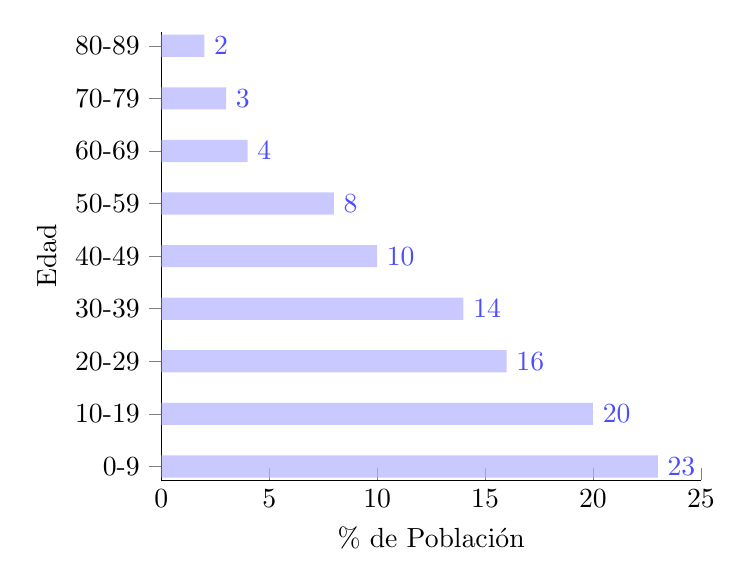
\begin{tikzpicture}
        \begin{axis}[
            xbar,
            xmin=0, xmax=25,
            ytick={0,10,...,90},
            yticklabels={0-9,10-19,20-29,30-39,40-49,50-59,60-69,70-79,80-89},
            xlabel={\% de Población},
            ylabel={Edad},
            bar width=8pt,
            enlarge y limits={abs=5pt},
            axis x line*=bottom,
            axis y line*=left,
            nodes near coords,
            every axis plot/.append style={
                fill=blue,
                draw=none,
                opacity=0.7
            }
        ]
    
        % Datos normalizados como porcentajes del total
        \addplot coordinates {(23,0) (20,10) (16,20) (14,30) (10,40) (8,50) (4,60) (3,70) (2,80)};
        
        \end{axis}
    \end{tikzpicture}
    \caption{Ejemplo de Pirámide de Edad}
    \label{fig:Pir_Edad}
\end{figure}

\begin{definicion}[Tasa de Crecimiento]
    Definimos la tasa de crecimiento asociada a una población $P_n$ en el periodo $n-$ésimo como:
    \begin{equation*}
        \frac{\|P_n\|-\|P_{n-1}\|}{\|P_{n-1}\|}
        = \frac{\|P_n\|}{\|P_{n-1}\|} -1
    \end{equation*}
\end{definicion}

\begin{definicion}[Tasa neta de reproducción]
    Se define la tasa neta de reproducción asociada a un modelo de Leslie dado como sigue:
    \begin{equation*}
        R := f_1 + p_1f_2 + p_1p_2f_3 + \ldots + p_1p_2\ldots p_{m-1}f_m
    \end{equation*}
    Este valor representa la tasa de fertilidad asociado a una hembra a lo largo de toda su vida.
\end{definicion}
Podríamos pensar que basta considerar simplemente: $R = \sum\limits_{k=1}^m f_k$, pero debemos tener en cuenta la probabilidad de cada individuo en llegar al grupo $k-$ésimo, antes de considerar la tasa de fertilidad del grupo $k$.\\

Una vez introducidos estos conceptos, procedemos al análisis del comportamiento asintótico, suponiendo que \textbf{$L$ tiene un valor propio dominante $\lm_i$}. La siguiente proposición nos proporcionará el valor de $v_{\lm_i}$.
\begin{prop}
    Consideramos la matriz de Leslie $L\in \cc{M}_m(\bb{R})$, y supongamos que $\lm_i$ es el valor propio dominante de $L$. Entonces, si notamos por $v_{\lm_i}(k)$ a la componente $k-$ésima del vector $v_{\lm_i}$, tenemos que $v_{\lm_i}(1)=1$ y:
    \begin{equation*}
        v_{\lm_i}(k) = \prod_{t=1}^{k-1} \frac{p_t}{\lm_i} = \dfrac{p_1\ldots p_{k-1}}{\lm_i^{k-1}} \qquad \forall k \in \{2, \ldots, m\}
    \end{equation*}
    
    Es decir, el vector propio asociado a $\lm_i$ es: 
    \begin{equation*}
        v_{\lm_i} = \begin{pmatrix}
            1 \\
            \dfrac{p_1}{\lm_i} \\
            \dfrac{p_1p_2}{\lm_i^2}\\
            \vdots\\
            \dfrac{p_1\dots p_{m-1}}{\lm_i^{m-1}}
        \end{pmatrix}
    \end{equation*}
    % // TODO: Cálculo del vector propio de leslie
    \begin{proof}
        Para determinar el vector $v_{\lm_i}$, resolvemos el sistema siguiente:
        \begin{equation*}
            Lv_{\lm_i} = \lm_i v_{\lm_i}
            \Longleftrightarrow
            (L-\lm_iId)v_{\lm_i} = 0
        \end{equation*}

        Tenemos entonces el siguiente sistema:
        \begin{equation*}
            \left\{
            \begin{array}{rcl}
                (f_1-\lm_i)v_{\lm_i}(1) + f_2v_{\lm_i}(2) + \dots + f_mv_{\lm_i}(m) &=& 0\\
                p_1v_{\lm_i}(1) -\lm_iv_{\lm_i}(2) &=& 0\\
                p_2v_{\lm_i}(2) -\lm_iv_{\lm_i}(3) &=& 0\\
                &\vdots&\\
                p_{m-1}v_{\lm_i}(m-1) -\lm_iv_{\lm_i}(m) &=&0
            \end{array}
            \right.
        \end{equation*}
        Como sabemos que el subespacio propio es de dimensión $1$ por ser la multiplicidad del valor propio dominante simple, podemos descartar la primera ecuación e imponer $v_{\lm_i}(1)=1$ (imponiendo otro valor nos saldría uno proporcional). Resolvemos ahora las soluciones en escalera, teniendo de forma directa el resultado buscado.
    \end{proof}
\end{prop}

Sabemos que:
\begin{equation*}
    \lim_{n\to \infty} \frac{P_n}{\lm_i^n} = \alpha v_{\lm_i} \qquad \alpha\in \bb{R}^+
\end{equation*}

Respecto a la pirámide de edad, tenemos que:
\begin{equation*}
    \lim_{n\to \infty} \frac{P_n}{\|P_n\|}
    = \lim_{n\to \infty} \frac{\alpha v_{\lm_i}\cdot |\lm_i|^n}{\|\alpha v_{\lm_i}\|\cdot \lm_i^n} = \frac{v_{\lm_i}}{\|v_{\lm_i}\|}
\end{equation*}
donde hemos empleado que la homogeneidad de la norma y que esta es una función continua.
Respecto a la tasa de crecimiento, tenemos que:
\begin{equation*}
    \lim_{n\to \infty} \frac{\|P_n\|}{\|P_{n-1}\|}-1
    = \lim_{n\to \infty} \frac{\|P_n\|}{\|P_{n-1}\|}\cdot \frac{\lm_i^{n-1}}{\lm_i^n}\cdot \lm_i-1
    = \lim_{n\to \infty} \frac{\|\alpha v_{\lm_i}\|}{\|\alpha v_{\lm_i}\|} \cdot \lm_i -1 = \lm_i-1
\end{equation*}

En resumen, tenemos que:
\begin{itemize}
    \item Si $\lm_i>1$: La población crece ilimitadamente.
    \item Si $\lm_i<1$: La población decrece y $\{P_n\}\to 0$; es decir, tiende a extinguirse.
    \item Si $\lm_i=1$: La población tiende a una población constante.
\end{itemize}
Además, la pirámide de edad a largo plazo es constante.\\

Notemos que todo este análisis se ha realizado suponiendo que hay un valor propio dominante; algo que no tenemos probado. Aunque podríamos pensar en usar el Teorema de Perron-Frobenious, no estamos en las hipótesis del enunciado, por lo que no es posible. La siguiente proposición nos es de gran ayuda.
\begin{prop}
    Dado un modelo de Leslie,
    si hay dos tasas de fertilidad $f_i$ consecutivas no nulas, entonces $L$ tiene valor propio dominante.
    \begin{proof}
    Veamos en primer lugar que $\exists !\lm_i\in \bb{R}$,~$\lm_i\neq 0$, tal que $\lm_i$ es un valor propio de $L$. Tenemos que $\lm_i$ es valor propio de $L$ si y solo si:
    \begin{align*}
        p(\lm_i) = 0 &\Longleftrightarrow \lm_i^m - f_1 \lm_i^{m-1} - f_2p_1\lm_i^{m-2} - \ldots - f_m p_1 \ldots p_{n-1} = 0 \\
        &\Longleftrightarrow \lm_i^m \left(1 - \dfrac{f_1}{\lm_i} - \dfrac{f_2p_1}{\lm_i^2} - \ldots - \dfrac{f_mp_1\ldots p_{m-1}}{\lm_i^m}\right) = 0
    \end{align*}
    
    Definimos ahora el polinomio dado por:
    \begin{equation*}
        q(\lm_i) = \dfrac{f_1}{\lm_i} + \dfrac{f_2p_1}{\lm_i^2} + \cdots + \dfrac{f_mp_1\ldots p_{m-1}}{\lm_i^m}
    \end{equation*}

    Por lo visto anteriormente, como $\lm_i\neq 0$, tenemos que:
    \begin{align*}
        p(\lm_i) = 0 &\Longleftrightarrow  \lm_i^m (1-q(\lm_i)) = 0 \\
        &\Longleftrightarrow q(\lm_i) = 1
    \end{align*}

    Tenemos que:
    \begin{equation*}
        \lim_{\lm\to 0^+}q(\lm) = +\infty
        \hspace{2cm}
        \lim_{\lm\to \infty}q(\lm) = 0
    \end{equation*}

    Por tanto, como $q$ es continua, tenemos que $\exists \lm_i\in \bb{R}^+$ tal que $q(\lm_i)=1$, por lo que tenemos demostrada la existencia buscada.
    Además, por la monotonía de $p$, tenemos que $\lm_i$ es único.
    Demostremos ahora que su multiplicidad es simple, es decir, que $p'(\lm_i)\neq 0$.
    \begin{equation*}
        p'(\lm) = m\lm^{m-1} (1-q(\lm)) - \lm^m q'(\lm)
        \Longrightarrow p'(\lm_i) = -\lm^m_i q'(\lm_i)
    \end{equation*}
    \begin{equation*}
        \left\{ \begin{array}{l}
            p(\lm_1) = 0 \\
            p'(\lm_1) = -\lm^m_1 q'(\lm_1) >0
        \end{array}\right.
    \end{equation*}
    donde hemos empleado que $q$ es estrictamente decreciente (pruébese).


    Tan solo nos falta por demostrar que si hay dos tasas consecutivas $f_i$ no nulas, entonces $|\lm|<\lm_i$ para todo $\lm\in \bb{C}$ tal que $p(\lm)=0$, $\lm\neq \lm_i$.
    % // TODO: Terminar Demostración de que es dominante
\end{proof}
\end{prop}

Veamos ahora qué relación hay entre la Tasa Neta de Reproducción $R$ y el valor propio dominante de la matriz de Leslie, $\lm_i$. Según la demostración de la proposición anterior, tenemos que $R=q(1)$, por lo que:
\begin{equation*}
    \lm_i > 1 \Longleftrightarrow R>1
\end{equation*}


\section{Aplicaciones a la genética}

\begin{ejemplo}
    Supongamos que tenemos un jardín con flores, cuyos fenotipos se codifican en genotipos de la siguiente manera:
    \begin{center}
        Rojas $(AA)$
        \hspace{1cm}
        Rosas $(Aa)$
        \hspace{1cm}
        Blancas $(aa)$
    \end{center}

    Usaremos la siguiente notación:
    \begin{itemize}
        \item Sea $x_n$ la proporción de flores rojas en el recuento $n$.
        \item Sea $y_n$ la proporción de flores rosas en el recuento $n$.
        \item Sea $z_n$ la proporción de flores blancas en el recuento $n$.
    \end{itemize}

    Supongamos que tan solo polinizamos con flores rojas $(AA)$. Tenemos que:
    \begin{itemize}
        \item El $100\%$ de las flores rojas producirán flores rojas al polinizarse con flores rojas.
        \item El $50\%$ de las flores rosas producirán flores rojas, mientras que el otro $50\%$ serán flores rosas, al polinizarse con flores rojas.
        \item El $100\%$ de las flores blancas producirán flores rosas al polinizarse con flores rojas.
    \end{itemize}

    Por tanto, tenemos el sistema $X_{n+1} = MX_n$, con:
    \begin{equation*}
        M = \begin{pmatrix}
            1 & \nicefrac{1}{2} & 0 \\
            0 & \nicefrac{1}{2} & 1 \\
            0 & 0 & 0 \\
        \end{pmatrix}
    \end{equation*}

    Tenemos que:
    \begin{equation*}
        \sigma(M) = \{1,\nicefrac{1}{2}, 0\} 
        \Longrightarrow
        \rho(M)=1
    \end{equation*}

    Por tanto, el valor propio dominante de $M$ es $\lm_i=1$. Calculemos su vector propio asociado:
    \begin{align*}
        V_1 &= \left\{(x,y,z)^t\in \bb{R}^3 \left|\begin{pmatrix}
            0 & \nicefrac{1}{2} & 0 \\
            0 & -\nicefrac{1}{2} & 1 \\
            0 & 0 & -1 \\
        \end{pmatrix}\begin{pmatrix}
            x\\y\\z
        \end{pmatrix}=0\right.\right\}
        = \cc{L}\left(\left\{\begin{pmatrix}
            1\\0\\0
        \end{pmatrix}\right\}\right)
    \end{align*}

    Por tanto, tenemos que:
    \begin{equation*}
        \lim_{n\to \infty} \frac{X_n}{1^n} = 
        \lim_{n\to \infty} X_n = \alpha \cdot \begin{pmatrix}
            1 \\ 0 \\ 0
        \end{pmatrix}
    \end{equation*}

    No obstante, por el concepto del problema, sabemos que $1=x_n+y_n+z_n$ para todo $n\in \bb{N}$, por lo que $\alpha=1$. De esta forma, tenemos que:
    \begin{equation*}
        \lim_{n\to \infty} X_n = \begin{pmatrix}
            1 \\ 0 \\ 0
        \end{pmatrix}
    \end{equation*}

    Por tanto, deducimos que la población de flores tenderá a estar formada solo por flores rojas.
\end{ejemplo}